\documentclass[1p]{elsarticle_modified}
%\bibliographystyle{elsarticle-num}

%\usepackage[colorlinks]{hyperref}
%\usepackage{abbrmath_seonhwa} %\Abb, \Ascr, \Acal ,\Abf, \Afrak
\usepackage{amsfonts}
\usepackage{amssymb}
\usepackage{amsmath}
\usepackage{amsthm}
\usepackage{scalefnt}
\usepackage{amsbsy}
\usepackage{kotex}
\usepackage{caption}
\usepackage{subfig}
\usepackage{color}
\usepackage{graphicx}
\usepackage{xcolor} %% white, black, red, green, blue, cyan, magenta, yellow
\usepackage{float}
\usepackage{setspace}
\usepackage{hyperref}

\usepackage{tikz}
\usetikzlibrary{arrows}

\usepackage{multirow}
\usepackage{array} % fixed length table
\usepackage{hhline}

%%%%%%%%%%%%%%%%%%%%%
\makeatletter
\renewcommand*\env@matrix[1][\arraystretch]{%
	\edef\arraystretch{#1}%
	\hskip -\arraycolsep
	\let\@ifnextchar\new@ifnextchar
	\array{*\c@MaxMatrixCols c}}
\makeatother %https://tex.stackexchange.com/questions/14071/how-can-i-increase-the-line-spacing-in-a-matrix
%%%%%%%%%%%%%%%

\usepackage[normalem]{ulem}

\newcommand{\msout}[1]{\ifmmode\text{\sout{\ensuremath{#1}}}\else\sout{#1}\fi}
%SOURCE: \msout is \stkout macro in https://tex.stackexchange.com/questions/20609/strikeout-in-math-mode

\newcommand{\cancel}[1]{
	\ifmmode
	{\color{red}\msout{#1}}
	\else
	{\color{red}\sout{#1}}
	\fi
}

\newcommand{\add}[1]{
	{\color{blue}\uwave{#1}}
}

\newcommand{\replace}[2]{
	\ifmmode
	{\color{red}\msout{#1}}{\color{blue}\uwave{#2}}
	\else
	{\color{red}\sout{#1}}{\color{blue}\uwave{#2}}
	\fi
}

\newcommand{\Sol}{\mathcal{S}} %segment
\newcommand{\D}{D} %diagram
\newcommand{\A}{\mathcal{A}} %arc


%%%%%%%%%%%%%%%%%%%%%%%%%%%%%5 test

\def\sl{\operatorname{\textup{SL}}(2,\Cbb)}
\def\psl{\operatorname{\textup{PSL}}(2,\Cbb)}
\def\quan{\mkern 1mu \triangleright \mkern 1mu}

\theoremstyle{definition}
\newtheorem{thm}{Theorem}[section]
\newtheorem{prop}[thm]{Proposition}
\newtheorem{lem}[thm]{Lemma}
\newtheorem{ques}[thm]{Question}
\newtheorem{cor}[thm]{Corollary}
\newtheorem{defn}[thm]{Definition}
\newtheorem{exam}[thm]{Example}
\newtheorem{rmk}[thm]{Remark}
\newtheorem{alg}[thm]{Algorithm}

\newcommand{\I}{\sqrt{-1}}
\begin{document}

%\begin{frontmatter}
%
%\title{Boundary parabolic representations of knots up to 8 crossings}
%
%%% Group authors per affiliation:
%\author{Yunhi Cho} 
%\address{Department of Mathematics, University of Seoul, Seoul, Korea}
%\ead{yhcho@uos.ac.kr}
%
%
%\author{Seonhwa Kim} %\fnref{s_kim}}
%\address{Center for Geometry and Physics, Institute for Basic Science, Pohang, 37673, Korea}
%\ead{ryeona17@ibs.re.kr}
%
%\author{Hyuk Kim}
%\address{Department of Mathematical Sciences, Seoul National University, Seoul 08826, Korea}
%\ead{hyukkim@snu.ac.kr}
%
%\author{Seokbeom Yoon}
%\address{Department of Mathematical Sciences, Seoul National University, Seoul, 08826,  Korea}
%\ead{sbyoon15@snu.ac.kr}
%
%\begin{abstract}
%We find all boundary parabolic representation of knots up to 8 crossings.
%
%\end{abstract}
%\begin{keyword}
%    \MSC[2010] 57M25 
%\end{keyword}
%
%\end{frontmatter}

%\linenumbers
%\tableofcontents
%
\newcommand\colored[1]{\textcolor{white}{\rule[-0.35ex]{0.8em}{1.4ex}}\kern-0.8em\color{red} #1}%
%\newcommand\colored[1]{\textcolor{white}{ #1}\kern-2.17ex	\textcolor{white}{ #1}\kern-1.81ex	\textcolor{white}{ #1}\kern-2.15ex\color{red}#1	}

{\Large $\underline{12a_{0815}~(K12a_{0815})}$}

\setlength{\tabcolsep}{10pt}
\renewcommand{\arraystretch}{1.6}
\vspace{1cm}\begin{tabular}{m{100pt}>{\centering\arraybackslash}m{274pt}}
\multirow{5}{120pt}{
	\centering
	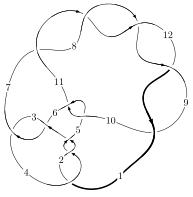
\includegraphics[width=112pt]{../../../GIT/diagram.site/Diagrams/png/1616_12a_0815.png}\\
\ \ \ A knot diagram\footnotemark}&
\allowdisplaybreaks
\textbf{Linearized knot diagam} \\
\cline{2-2}
 &
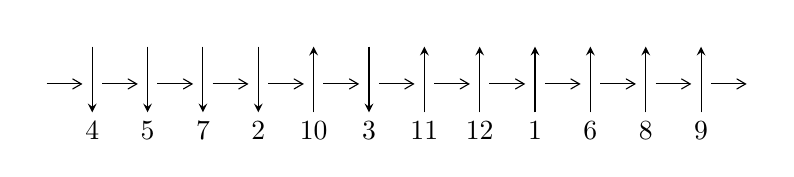
\begin{tikzpicture}[x=20pt, y=17pt]
	% nodes
	\node (C0) at (0, 0) {};
	\node (C1) at (1, 0) {};
	\node (C1U) at (1, +1) {};
	\node (C1D) at (1, -1) {4};

	\node (C2) at (2, 0) {};
	\node (C2U) at (2, +1) {};
	\node (C2D) at (2, -1) {5};

	\node (C3) at (3, 0) {};
	\node (C3U) at (3, +1) {};
	\node (C3D) at (3, -1) {7};

	\node (C4) at (4, 0) {};
	\node (C4U) at (4, +1) {};
	\node (C4D) at (4, -1) {2};

	\node (C5) at (5, 0) {};
	\node (C5U) at (5, +1) {};
	\node (C5D) at (5, -1) {10};

	\node (C6) at (6, 0) {};
	\node (C6U) at (6, +1) {};
	\node (C6D) at (6, -1) {3};

	\node (C7) at (7, 0) {};
	\node (C7U) at (7, +1) {};
	\node (C7D) at (7, -1) {11};

	\node (C8) at (8, 0) {};
	\node (C8U) at (8, +1) {};
	\node (C8D) at (8, -1) {12};

	\node (C9) at (9, 0) {};
	\node (C9U) at (9, +1) {};
	\node (C9D) at (9, -1) {1};

	\node (C10) at (10, 0) {};
	\node (C10U) at (10, +1) {};
	\node (C10D) at (10, -1) {6};

	\node (C11) at (11, 0) {};
	\node (C11U) at (11, +1) {};
	\node (C11D) at (11, -1) {8};

	\node (C12) at (12, 0) {};
	\node (C12U) at (12, +1) {};
	\node (C12D) at (12, -1) {9};
	\node (C13) at (13, 0) {};

	% arrows
	\draw[->,>={angle 60}]
	(C0) edge (C1) (C1) edge (C2) (C2) edge (C3) (C3) edge (C4) (C4) edge (C5) (C5) edge (C6) (C6) edge (C7) (C7) edge (C8) (C8) edge (C9) (C9) edge (C10) (C10) edge (C11) (C11) edge (C12) (C12) edge (C13) ;	\draw[->,>=stealth]
	(C1U) edge (C1D) (C2U) edge (C2D) (C3U) edge (C3D) (C4U) edge (C4D) (C5D) edge (C5U) (C6U) edge (C6D) (C7D) edge (C7U) (C8D) edge (C8U) (C9D) edge (C9U) (C10D) edge (C10U) (C11D) edge (C11U) (C12D) edge (C12U) ;
	\end{tikzpicture} \\
\hhline{~~} \\& 
\textbf{Solving Sequence} \\ \cline{2-2} 
 &
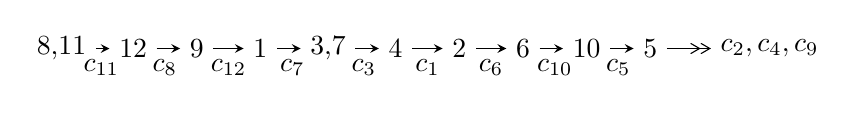
\begin{tikzpicture}[x=23pt, y=7pt]
	% node
	\node (A0) at (-1/8, 0) {8,11};
	\node (A1) at (1, 0) {12};
	\node (A2) at (2, 0) {9};
	\node (A3) at (3, 0) {1};
	\node (A4) at (65/16, 0) {3,7};
	\node (A5) at (41/8, 0) {4};
	\node (A6) at (49/8, 0) {2};
	\node (A7) at (57/8, 0) {6};
	\node (A8) at (65/8, 0) {10};
	\node (A9) at (73/8, 0) {5};
	\node (C1) at (1/2, -1) {$c_{11}$};
	\node (C2) at (3/2, -1) {$c_{8}$};
	\node (C3) at (5/2, -1) {$c_{12}$};
	\node (C4) at (7/2, -1) {$c_{7}$};
	\node (C5) at (37/8, -1) {$c_{3}$};
	\node (C6) at (45/8, -1) {$c_{1}$};
	\node (C7) at (53/8, -1) {$c_{6}$};
	\node (C8) at (61/8, -1) {$c_{10}$};
	\node (C9) at (69/8, -1) {$c_{5}$};
	\node (A10) at (11, 0) {$c_{2},c_{4},c_{9}$};

	% edge
	\draw[->,>=stealth]	
	(A0) edge (A1) (A1) edge (A2) (A2) edge (A3) (A3) edge (A4) (A4) edge (A5) (A5) edge (A6) (A6) edge (A7) (A7) edge (A8) (A8) edge (A9) ;
	\draw[->>,>={angle 60}]	
	(A9) edge (A10);
\end{tikzpicture} \\ 

\end{tabular} \\

\footnotetext{
The image of knot diagram is generated by the software ``\textbf{Draw programme}" developed by Andrew Bartholomew(\url{http://www.layer8.co.uk/maths/draw/index.htm\#Running-draw}), where we modified some parts for our purpose(\url{https://github.com/CATsTAILs/LinksPainter}).
}\phantom \\ \newline 
\centering \textbf{Ideals for irreducible components\footnotemark of $X_{\text{par}}$} 
 
\begin{align*}
I^u_{1}&=\langle 
-1.39811\times10^{17} u^{53}+3.48531\times10^{17} u^{52}+\cdots+3.74793\times10^{16} b+1.64653\times10^{17},\\
\phantom{I^u_{1}}&\phantom{= \langle  }6.79652\times10^{16} u^{53}-2.14430\times10^{17} u^{52}+\cdots+3.74793\times10^{16} a-3.66519\times10^{17},\;u^{54}-4 u^{53}+\cdots-12 u+1\rangle \\
I^u_{2}&=\langle 
u^2+b- u-2,\;- u^2+a+u+2,\;u^3- u^2-2 u+1\rangle \\
I^u_{3}&=\langle 
b+u-1,\;a+3,\;u^2+u-1\rangle \\
I^u_{4}&=\langle 
b+1,\;a-2,\;u^2+u-1\rangle \\
\\
\end{align*}
\raggedright * 4 irreducible components of $\dim_{\mathbb{C}}=0$, with total 61 representations.\\
\footnotetext{All coefficients of polynomials are rational numbers. But the coefficients are sometimes approximated in decimal forms when there is not enough margin.}
\newpage
\renewcommand{\arraystretch}{1}
\centering \section*{I. $I^u_{1}= \langle -1.40\times10^{17} u^{53}+3.49\times10^{17} u^{52}+\cdots+3.75\times10^{16} b+1.65\times10^{17},\;6.80\times10^{16} u^{53}-2.14\times10^{17} u^{52}+\cdots+3.75\times10^{16} a-3.67\times10^{17},\;u^{54}-4 u^{53}+\cdots-12 u+1 \rangle$}
\flushleft \textbf{(i) Arc colorings}\\
\begin{tabular}{m{7pt} m{180pt} m{7pt} m{180pt} }
\flushright $a_{8}=$&$\begin{pmatrix}0\\u\end{pmatrix}$ \\
\flushright $a_{11}=$&$\begin{pmatrix}1\\0\end{pmatrix}$ \\
\flushright $a_{12}=$&$\begin{pmatrix}1\\- u^2\end{pmatrix}$ \\
\flushright $a_{9}=$&$\begin{pmatrix}u\\- u^3+u\end{pmatrix}$ \\
\flushright $a_{1}=$&$\begin{pmatrix}- u^2+1\\u^4-2 u^2\end{pmatrix}$ \\
\flushright $a_{3}=$&$\begin{pmatrix}-1.81341 u^{53}+5.72128 u^{52}+\cdots-57.8240 u+9.77923\\3.73034 u^{53}-9.29930 u^{52}+\cdots+36.1231 u-4.39318\end{pmatrix}$ \\
\flushright $a_{7}=$&$\begin{pmatrix}- u\\u\end{pmatrix}$ \\
\flushright $a_{4}=$&$\begin{pmatrix}-9.13774 u^{53}+22.8480 u^{52}+\cdots-104.984 u+13.8690\\11.0547 u^{53}-26.4260 u^{52}+\cdots+83.2829 u-8.48291\end{pmatrix}$ \\
\flushright $a_{2}=$&$\begin{pmatrix}11.7271 u^{53}-28.5773 u^{52}+\cdots+105.648 u-12.1490\\-11.8102 u^{53}+27.9993 u^{52}+\cdots-86.3491 u+8.53503\end{pmatrix}$ \\
\flushright $a_{6}=$&$\begin{pmatrix}-4.40884 u^{53}+10.2375 u^{52}+\cdots-46.3267 u+6.19547\\6.42322 u^{53}-15.2092 u^{52}+\cdots+47.7853 u-4.63561\end{pmatrix}$ \\
\flushright $a_{10}=$&$\begin{pmatrix}- u^3+2 u\\u^5-3 u^3+u\end{pmatrix}$ \\
\flushright $a_{5}=$&$\begin{pmatrix}6.54314 u^{53}-14.0720 u^{52}+\cdots+18.5879 u+0.684875\\-6.46008 u^{53}+14.6500 u^{52}+\cdots-37.8870 u+2.92907\end{pmatrix}$\\&\end{tabular}
\flushleft \textbf{(ii) Obstruction class $= -1$}\\~\\
\flushleft \textbf{(iii) Cusp Shapes $= \frac{363185510972410645}{37479301199371286} u^{53}-\frac{688675840018976189}{18739650599685643} u^{52}+\cdots+\frac{4805743652784223102}{18739650599685643} u-\frac{1430274773919045159}{37479301199371286}$}\\~\\
\newpage\renewcommand{\arraystretch}{1}
\flushleft \textbf{(iv) u-Polynomials at the component}\newline \\
\begin{tabular}{m{50pt}|m{274pt}}
Crossings & \hspace{64pt}u-Polynomials at each crossing \\
\hline $$\begin{aligned}c_{1},c_{2},c_{4}\end{aligned}$$&$\begin{aligned}
&u^{54}-6 u^{53}+\cdots-37 u-1
\end{aligned}$\\
\hline $$\begin{aligned}c_{3},c_{6}\end{aligned}$$&$\begin{aligned}
&u^{54}+3 u^{53}+\cdots-4 u+8
\end{aligned}$\\
\hline $$\begin{aligned}c_{5},c_{10}\end{aligned}$$&$\begin{aligned}
&u^{54}+2 u^{53}+\cdots-64 u-16
\end{aligned}$\\
\hline $$\begin{aligned}c_{7},c_{8},c_{9}\\c_{11},c_{12}\end{aligned}$$&$\begin{aligned}
&u^{54}-4 u^{53}+\cdots-12 u+1
\end{aligned}$\\
\hline
\end{tabular}\\~\\
\newpage\renewcommand{\arraystretch}{1}
\flushleft \textbf{(v) Riley Polynomials at the component}\newline \\
\begin{tabular}{m{50pt}|m{274pt}}
Crossings & \hspace{64pt}Riley Polynomials at each crossing \\
\hline $$\begin{aligned}c_{1},c_{2},c_{4}\end{aligned}$$&$\begin{aligned}
&y^{54}-50 y^{53}+\cdots-985 y+1
\end{aligned}$\\
\hline $$\begin{aligned}c_{3},c_{6}\end{aligned}$$&$\begin{aligned}
&y^{54}-27 y^{53}+\cdots-3088 y+64
\end{aligned}$\\
\hline $$\begin{aligned}c_{5},c_{10}\end{aligned}$$&$\begin{aligned}
&y^{54}-30 y^{53}+\cdots-7808 y+256
\end{aligned}$\\
\hline $$\begin{aligned}c_{7},c_{8},c_{9}\\c_{11},c_{12}\end{aligned}$$&$\begin{aligned}
&y^{54}-72 y^{53}+\cdots-24 y+1
\end{aligned}$\\
\hline
\end{tabular}\\~\\
\newpage\flushleft \textbf{(vi) Complex Volumes and Cusp Shapes}
$$\begin{array}{c|c|c}  
\text{Solutions to }I^u_{1}& \I (\text{vol} + \sqrt{-1}CS) & \text{Cusp shape}\\
 \hline 
\begin{aligned}
u &= -0.955893 + 0.280895 I \\
a &= -0.657144 + 0.964305 I \\
b &= -0.167798 + 0.004865 I\end{aligned}
 & \phantom{-}0.99214 - 4.46696 I & \phantom{-0.000000 } 0 \\ \hline\begin{aligned}
u &= -0.955893 - 0.280895 I \\
a &= -0.657144 - 0.964305 I \\
b &= -0.167798 - 0.004865 I\end{aligned}
 & \phantom{-}0.99214 + 4.46696 I & \phantom{-0.000000 } 0 \\ \hline\begin{aligned}
u &= -0.954075 + 0.196551 I \\
a &= -2.44568 + 0.32192 I \\
b &= \phantom{-}1.39296 - 0.94545 I\end{aligned}
 & \phantom{-}1.98617 - 1.55786 I & \phantom{-0.000000 } 0 \\ \hline\begin{aligned}
u &= -0.954075 - 0.196551 I \\
a &= -2.44568 - 0.32192 I \\
b &= \phantom{-}1.39296 + 0.94545 I\end{aligned}
 & \phantom{-}1.98617 + 1.55786 I & \phantom{-0.000000 } 0 \\ \hline\begin{aligned}
u &= -1.003860 + 0.333824 I \\
a &= \phantom{-}1.98014 - 0.51608 I \\
b &= -1.15335 + 1.40699 I\end{aligned}
 & \phantom{-}4.09810 - 6.73935 I & \phantom{-0.000000 } 0 \\ \hline\begin{aligned}
u &= -1.003860 - 0.333824 I \\
a &= \phantom{-}1.98014 + 0.51608 I \\
b &= -1.15335 - 1.40699 I\end{aligned}
 & \phantom{-}4.09810 + 6.73935 I & \phantom{-0.000000 } 0 \\ \hline\begin{aligned}
u &= \phantom{-}1.037550 + 0.306742 I \\
a &= -0.949401 - 0.673804 I \\
b &= \phantom{-}0.037724 + 1.330030 I\end{aligned}
 & -3.90243 + 4.30298 I & \phantom{-0.000000 } 0 \\ \hline\begin{aligned}
u &= \phantom{-}1.037550 - 0.306742 I \\
a &= -0.949401 + 0.673804 I \\
b &= \phantom{-}0.037724 - 1.330030 I\end{aligned}
 & -3.90243 - 4.30298 I & \phantom{-0.000000 } 0 \\ \hline\begin{aligned}
u &= -1.004380 + 0.437767 I \\
a &= -1.67226 + 0.47123 I \\
b &= \phantom{-}0.92436 - 1.53705 I\end{aligned}
 & -1.30619 - 11.23270 I & \phantom{-0.000000 } 0 \\ \hline\begin{aligned}
u &= -1.004380 - 0.437767 I \\
a &= -1.67226 - 0.47123 I \\
b &= \phantom{-}0.92436 + 1.53705 I\end{aligned}
 & -1.30619 + 11.23270 I & \phantom{-0.000000 } 0\\
 \hline 
 \end{array}$$\newpage$$\begin{array}{c|c|c}  
\text{Solutions to }I^u_{1}& \I (\text{vol} + \sqrt{-1}CS) & \text{Cusp shape}\\
 \hline 
\begin{aligned}
u &= \phantom{-}0.889050 + 0.150577 I \\
a &= \phantom{-}0.895885 + 0.803841 I \\
b &= -0.126696 - 1.360540 I\end{aligned}
 & \phantom{-}1.36794 + 1.65747 I & \phantom{-}6.44317 - 4.64193 I \\ \hline\begin{aligned}
u &= \phantom{-}0.889050 - 0.150577 I \\
a &= \phantom{-}0.895885 - 0.803841 I \\
b &= -0.126696 + 1.360540 I\end{aligned}
 & \phantom{-}1.36794 - 1.65747 I & \phantom{-}6.44317 + 4.64193 I \\ \hline\begin{aligned}
u &= -1.113440 + 0.153181 I \\
a &= \phantom{-}0.382959 - 0.729976 I \\
b &= \phantom{-}0.0606512 + 0.0742692 I\end{aligned}
 & \phantom{-}6.28050 - 1.40683 I & \phantom{-0.000000 } 0 \\ \hline\begin{aligned}
u &= -1.113440 - 0.153181 I \\
a &= \phantom{-}0.382959 + 0.729976 I \\
b &= \phantom{-}0.0606512 - 0.0742692 I\end{aligned}
 & \phantom{-}6.28050 + 1.40683 I & \phantom{-0.000000 } 0 \\ \hline\begin{aligned}
u &= \phantom{-}0.647324 + 0.583844 I \\
a &= \phantom{-}1.140030 + 0.621418 I \\
b &= \phantom{-}0.132989 - 1.059230 I\end{aligned}
 & -3.55059 - 3.17785 I & \phantom{-}2.00000 + 1.62776 I \\ \hline\begin{aligned}
u &= \phantom{-}0.647324 - 0.583844 I \\
a &= \phantom{-}1.140030 - 0.621418 I \\
b &= \phantom{-}0.132989 + 1.059230 I\end{aligned}
 & -3.55059 + 3.17785 I & \phantom{-}2.00000 - 1.62776 I \\ \hline\begin{aligned}
u &= \phantom{-}0.708312 + 0.161436 I \\
a &= -0.110891 + 1.210160 I \\
b &= -0.21103 - 1.94212 I\end{aligned}
 & -0.861342 + 0.425422 I & \phantom{-}8.90403 + 2.84052 I \\ \hline\begin{aligned}
u &= \phantom{-}0.708312 - 0.161436 I \\
a &= -0.110891 - 1.210160 I \\
b &= -0.21103 + 1.94212 I\end{aligned}
 & -0.861342 - 0.425422 I & \phantom{-}8.90403 - 2.84052 I \\ \hline\begin{aligned}
u &= -0.724781\phantom{ +0.000000I} \\
a &= \phantom{-}3.04269\phantom{ +0.000000I} \\
b &= -0.702104\phantom{ +0.000000I}\end{aligned}
 & -7.67173\phantom{ +0.000000I} & \phantom{-}19.8130\phantom{ +0.000000I} \\ \hline\begin{aligned}
u &= \phantom{-}0.180101 + 0.700187 I \\
a &= \phantom{-}0.088171 - 0.373846 I \\
b &= -0.49531 - 1.40016 I\end{aligned}
 & -4.94514 + 7.40203 I & -1.00662 - 6.28181 I\\
 \hline 
 \end{array}$$\newpage$$\begin{array}{c|c|c}  
\text{Solutions to }I^u_{1}& \I (\text{vol} + \sqrt{-1}CS) & \text{Cusp shape}\\
 \hline 
\begin{aligned}
u &= \phantom{-}0.180101 - 0.700187 I \\
a &= \phantom{-}0.088171 + 0.373846 I \\
b &= -0.49531 + 1.40016 I\end{aligned}
 & -4.94514 - 7.40203 I & -1.00662 + 6.28181 I \\ \hline\begin{aligned}
u &= \phantom{-}0.484782 + 0.418903 I \\
a &= -1.25208 - 0.74775 I \\
b &= -0.023304 + 0.876278 I\end{aligned}
 & \phantom{-}1.232030 - 0.400002 I & \phantom{-}7.11175 + 0.11005 I \\ \hline\begin{aligned}
u &= \phantom{-}0.484782 - 0.418903 I \\
a &= -1.25208 + 0.74775 I \\
b &= -0.023304 - 0.876278 I\end{aligned}
 & \phantom{-}1.232030 + 0.400002 I & \phantom{-}7.11175 - 0.11005 I \\ \hline\begin{aligned}
u &= \phantom{-}0.212049 + 0.561353 I \\
a &= -0.355668 + 0.444206 I \\
b &= \phantom{-}0.58234 + 1.33649 I\end{aligned}
 & \phantom{-}0.34502 + 3.69748 I & \phantom{-}2.76292 - 6.81307 I \\ \hline\begin{aligned}
u &= \phantom{-}0.212049 - 0.561353 I \\
a &= -0.355668 - 0.444206 I \\
b &= \phantom{-}0.58234 - 1.33649 I\end{aligned}
 & \phantom{-}0.34502 - 3.69748 I & \phantom{-}2.76292 + 6.81307 I \\ \hline\begin{aligned}
u &= -0.281238 + 0.495314 I \\
a &= \phantom{-}0.769983 + 1.023740 I \\
b &= \phantom{-}0.106414 + 1.105760 I\end{aligned}
 & -7.98083 - 1.54477 I & -5.36049 + 2.77593 I \\ \hline\begin{aligned}
u &= -0.281238 - 0.495314 I \\
a &= \phantom{-}0.769983 - 1.023740 I \\
b &= \phantom{-}0.106414 - 1.105760 I\end{aligned}
 & -7.98083 + 1.54477 I & -5.36049 - 2.77593 I \\ \hline\begin{aligned}
u &= -1.45229 + 0.18721 I \\
a &= -0.812390 + 0.483425 I \\
b &= \phantom{-}0.156984 - 0.422947 I\end{aligned}
 & \phantom{-}3.36449 + 0.31719 I & \phantom{-0.000000 } 0 \\ \hline\begin{aligned}
u &= -1.45229 - 0.18721 I \\
a &= -0.812390 - 0.483425 I \\
b &= \phantom{-}0.156984 + 0.422947 I\end{aligned}
 & \phantom{-}3.36449 - 0.31719 I & \phantom{-0.000000 } 0 \\ \hline\begin{aligned}
u &= \phantom{-}0.139977 + 0.472620 I \\
a &= \phantom{-}1.76198 + 0.54098 I \\
b &= \phantom{-}0.201388 - 0.650535 I\end{aligned}
 & -2.37654 + 1.88570 I & -0.67343 - 3.61371 I\\
 \hline 
 \end{array}$$\newpage$$\begin{array}{c|c|c}  
\text{Solutions to }I^u_{1}& \I (\text{vol} + \sqrt{-1}CS) & \text{Cusp shape}\\
 \hline 
\begin{aligned}
u &= \phantom{-}0.139977 - 0.472620 I \\
a &= \phantom{-}1.76198 - 0.54098 I \\
b &= \phantom{-}0.201388 + 0.650535 I\end{aligned}
 & -2.37654 - 1.88570 I & -0.67343 + 3.61371 I \\ \hline\begin{aligned}
u &= \phantom{-}0.487736\phantom{ +0.000000I} \\
a &= -0.807237\phantom{ +0.000000I} \\
b &= \phantom{-}0.441336\phantom{ +0.000000I}\end{aligned}
 & \phantom{-}0.740706\phantom{ +0.000000I} & \phantom{-}13.6380\phantom{ +0.000000I} \\ \hline\begin{aligned}
u &= -1.60169\phantom{ +0.000000I} \\
a &= \phantom{-}2.38830\phantom{ +0.000000I} \\
b &= -2.02710\phantom{ +0.000000I}\end{aligned}
 & \phantom{-}8.10579\phantom{ +0.000000I} & \phantom{-0.000000 } 0 \\ \hline\begin{aligned}
u &= -1.65983 + 0.02504 I \\
a &= \phantom{-}0.87862 + 1.94748 I \\
b &= -0.58285 - 2.35560 I\end{aligned}
 & \phantom{-}7.60543 - 1.00097 I & \phantom{-0.000000 } 0 \\ \hline\begin{aligned}
u &= -1.65983 - 0.02504 I \\
a &= \phantom{-}0.87862 - 1.94748 I \\
b &= -0.58285 + 2.35560 I\end{aligned}
 & \phantom{-}7.60543 + 1.00097 I & \phantom{-0.000000 } 0 \\ \hline\begin{aligned}
u &= \phantom{-}1.66740\phantom{ +0.000000I} \\
a &= -2.44614\phantom{ +0.000000I} \\
b &= \phantom{-}1.33681\phantom{ +0.000000I}\end{aligned}
 & \phantom{-}0.921274\phantom{ +0.000000I} & \phantom{-0.000000 } 0 \\ \hline\begin{aligned}
u &= -1.69751 + 0.03635 I \\
a &= -0.96750 + 1.32403 I \\
b &= \phantom{-}0.48614 - 1.68807 I\end{aligned}
 & \phantom{-}10.60180 - 2.36821 I & \phantom{-0.000000 } 0 \\ \hline\begin{aligned}
u &= -1.69751 - 0.03635 I \\
a &= -0.96750 - 1.32403 I \\
b &= \phantom{-}0.48614 + 1.68807 I\end{aligned}
 & \phantom{-}10.60180 + 2.36821 I & \phantom{-0.000000 } 0 \\ \hline\begin{aligned}
u &= \phantom{-}1.70775 + 0.07197 I \\
a &= \phantom{-}0.258719 + 0.302731 I \\
b &= \phantom{-}0.129943 + 0.458522 I\end{aligned}
 & \phantom{-}10.43440 + 5.86156 I & \phantom{-0.000000 } 0 \\ \hline\begin{aligned}
u &= \phantom{-}1.70775 - 0.07197 I \\
a &= \phantom{-}0.258719 - 0.302731 I \\
b &= \phantom{-}0.129943 - 0.458522 I\end{aligned}
 & \phantom{-}10.43440 - 5.86156 I & \phantom{-0.000000 } 0\\
 \hline 
 \end{array}$$\newpage$$\begin{array}{c|c|c}  
\text{Solutions to }I^u_{1}& \I (\text{vol} + \sqrt{-1}CS) & \text{Cusp shape}\\
 \hline 
\begin{aligned}
u &= \phantom{-}1.70917 + 0.05180 I \\
a &= \phantom{-}2.59054 + 0.66443 I \\
b &= -1.81746 - 0.96175 I\end{aligned}
 & \phantom{-}11.47430 + 2.55306 I & \phantom{-0.000000 } 0 \\ \hline\begin{aligned}
u &= \phantom{-}1.70917 - 0.05180 I \\
a &= \phantom{-}2.59054 - 0.66443 I \\
b &= -1.81746 + 0.96175 I\end{aligned}
 & \phantom{-}11.47430 - 2.55306 I & \phantom{-0.000000 } 0 \\ \hline\begin{aligned}
u &= \phantom{-}0.043095 + 0.280243 I \\
a &= \phantom{-}0.89056 - 1.82691 I \\
b &= -0.611450 - 0.877287 I\end{aligned}
 & -1.250130 - 0.131994 I & -5.38771 - 0.73638 I \\ \hline\begin{aligned}
u &= \phantom{-}0.043095 - 0.280243 I \\
a &= \phantom{-}0.89056 + 1.82691 I \\
b &= -0.611450 + 0.877287 I\end{aligned}
 & -1.250130 + 0.131994 I & -5.38771 + 0.73638 I \\ \hline\begin{aligned}
u &= \phantom{-}1.71938 + 0.08814 I \\
a &= -2.28411 - 1.00360 I \\
b &= \phantom{-}1.57801 + 1.44618 I\end{aligned}
 & \phantom{-}13.7389 + 8.4458 I & \phantom{-0.000000 } 0 \\ \hline\begin{aligned}
u &= \phantom{-}1.71938 - 0.08814 I \\
a &= -2.28411 + 1.00360 I \\
b &= \phantom{-}1.57801 - 1.44618 I\end{aligned}
 & \phantom{-}13.7389 - 8.4458 I & \phantom{-0.000000 } 0 \\ \hline\begin{aligned}
u &= \phantom{-}1.71805 + 0.12084 I \\
a &= \phantom{-}1.98176 + 1.07195 I \\
b &= -1.28426 - 1.61703 I\end{aligned}
 & \phantom{-}8.2449 + 13.5020 I & \phantom{-0.000000 } 0 \\ \hline\begin{aligned}
u &= \phantom{-}1.71805 - 0.12084 I \\
a &= \phantom{-}1.98176 - 1.07195 I \\
b &= -1.28426 + 1.61703 I\end{aligned}
 & \phantom{-}8.2449 - 13.5020 I & \phantom{-0.000000 } 0 \\ \hline\begin{aligned}
u &= -1.72791 + 0.08472 I \\
a &= \phantom{-}0.849535 - 1.106390 I \\
b &= -0.25652 + 1.47457 I\end{aligned}
 & \phantom{-}5.92114 - 5.92817 I & \phantom{-0.000000 } 0 \\ \hline\begin{aligned}
u &= -1.72791 - 0.08472 I \\
a &= \phantom{-}0.849535 + 1.106390 I \\
b &= -0.25652 - 1.47457 I\end{aligned}
 & \phantom{-}5.92114 + 5.92817 I & \phantom{-0.000000 } 0\\
 \hline 
 \end{array}$$\newpage$$\begin{array}{c|c|c}  
\text{Solutions to }I^u_{1}& \I (\text{vol} + \sqrt{-1}CS) & \text{Cusp shape}\\
 \hline 
\begin{aligned}
u &= \phantom{-}1.74587 + 0.03327 I \\
a &= -0.107778 - 0.244366 I \\
b &= -0.087691 - 0.343352 I\end{aligned}
 & \phantom{-}16.5619 + 2.1570 I & \phantom{-0.000000 } 0 \\ \hline\begin{aligned}
u &= \phantom{-}1.74587 - 0.03327 I \\
a &= -0.107778 + 0.244366 I \\
b &= -0.087691 + 0.343352 I\end{aligned}
 & \phantom{-}16.5619 - 2.1570 I & \phantom{-0.000000 } 0 \\ \hline\begin{aligned}
u &= \phantom{-}1.82048\phantom{ +0.000000I} \\
a &= \phantom{-}0.109703\phantom{ +0.000000I} \\
b &= \phantom{-}0.193921\phantom{ +0.000000I}\end{aligned}
 & \phantom{-}15.6372\phantom{ +0.000000I} & \phantom{-0.000000 } 0 \\ \hline\begin{aligned}
u &= \phantom{-}0.166814\phantom{ +0.000000I} \\
a &= \phantom{-}4.00471\phantom{ +0.000000I} \\
b &= -1.18722\phantom{ +0.000000I}\end{aligned}
 & -1.16691\phantom{ +0.000000I} & -12.8120\phantom{ +0.000000I}\\
 \hline 
 \end{array}$$\newpage\newpage\renewcommand{\arraystretch}{1}
\centering \section*{II. $I^u_{2}= \langle u^2+b- u-2,\;- u^2+a+u+2,\;u^3- u^2-2 u+1 \rangle$}
\flushleft \textbf{(i) Arc colorings}\\
\begin{tabular}{m{7pt} m{180pt} m{7pt} m{180pt} }
\flushright $a_{8}=$&$\begin{pmatrix}0\\u\end{pmatrix}$ \\
\flushright $a_{11}=$&$\begin{pmatrix}1\\0\end{pmatrix}$ \\
\flushright $a_{12}=$&$\begin{pmatrix}1\\- u^2\end{pmatrix}$ \\
\flushright $a_{9}=$&$\begin{pmatrix}u\\- u^2- u+1\end{pmatrix}$ \\
\flushright $a_{1}=$&$\begin{pmatrix}- u^2+1\\u^2+u-1\end{pmatrix}$ \\
\flushright $a_{3}=$&$\begin{pmatrix}u^2- u-2\\- u^2+u+2\end{pmatrix}$ \\
\flushright $a_{7}=$&$\begin{pmatrix}- u\\u\end{pmatrix}$ \\
\flushright $a_{4}=$&$\begin{pmatrix}u^2- u-2\\- u^2+u+2\end{pmatrix}$ \\
\flushright $a_{2}=$&$\begin{pmatrix}- u-1\\2 u+1\end{pmatrix}$ \\
\flushright $a_{6}=$&$\begin{pmatrix}- u\\u\end{pmatrix}$ \\
\flushright $a_{10}=$&$\begin{pmatrix}- u^2+1\\u^2\end{pmatrix}$ \\
\flushright $a_{5}=$&$\begin{pmatrix}u^2-1\\- u^2- u+1\end{pmatrix}$\\&\end{tabular}
\flushleft \textbf{(ii) Obstruction class $= 1$}\\~\\
\flushleft \textbf{(iii) Cusp Shapes $= -8 u^2+7 u+30$}\\~\\
\newpage\renewcommand{\arraystretch}{1}
\flushleft \textbf{(iv) u-Polynomials at the component}\newline \\
\begin{tabular}{m{50pt}|m{274pt}}
Crossings & \hspace{64pt}u-Polynomials at each crossing \\
\hline $$\begin{aligned}c_{1},c_{2}\end{aligned}$$&$\begin{aligned}
&(u-1)^3
\end{aligned}$\\
\hline $$\begin{aligned}c_{3},c_{6}\end{aligned}$$&$\begin{aligned}
&u^3
\end{aligned}$\\
\hline $$\begin{aligned}c_{4}\end{aligned}$$&$\begin{aligned}
&(u+1)^3
\end{aligned}$\\
\hline $$\begin{aligned}c_{5},c_{7},c_{8}\\c_{9}\end{aligned}$$&$\begin{aligned}
&u^3+u^2-2 u-1
\end{aligned}$\\
\hline $$\begin{aligned}c_{10},c_{11},c_{12}\end{aligned}$$&$\begin{aligned}
&u^3- u^2-2 u+1
\end{aligned}$\\
\hline
\end{tabular}\\~\\
\newpage\renewcommand{\arraystretch}{1}
\flushleft \textbf{(v) Riley Polynomials at the component}\newline \\
\begin{tabular}{m{50pt}|m{274pt}}
Crossings & \hspace{64pt}Riley Polynomials at each crossing \\
\hline $$\begin{aligned}c_{1},c_{2},c_{4}\end{aligned}$$&$\begin{aligned}
&(y-1)^3
\end{aligned}$\\
\hline $$\begin{aligned}c_{3},c_{6}\end{aligned}$$&$\begin{aligned}
&y^3
\end{aligned}$\\
\hline $$\begin{aligned}c_{5},c_{7},c_{8}\\c_{9},c_{10},c_{11}\\c_{12}\end{aligned}$$&$\begin{aligned}
&y^3-5 y^2+6 y-1
\end{aligned}$\\
\hline
\end{tabular}\\~\\
\newpage\flushleft \textbf{(vi) Complex Volumes and Cusp Shapes}
$$\begin{array}{c|c|c}  
\text{Solutions to }I^u_{2}& \I (\text{vol} + \sqrt{-1}CS) & \text{Cusp shape}\\
 \hline 
\begin{aligned}
u &= -1.24698\phantom{ +0.000000I} \\
a &= \phantom{-}0.801938\phantom{ +0.000000I} \\
b &= -0.801938\phantom{ +0.000000I}\end{aligned}
 & \phantom{-}4.69981\phantom{ +0.000000I} & \phantom{-}8.83150\phantom{ +0.000000I} \\ \hline\begin{aligned}
u &= \phantom{-}0.445042\phantom{ +0.000000I} \\
a &= -2.24698\phantom{ +0.000000I} \\
b &= \phantom{-}2.24698\phantom{ +0.000000I}\end{aligned}
 & -0.939962\phantom{ +0.000000I} & \phantom{-}31.5310\phantom{ +0.000000I} \\ \hline\begin{aligned}
u &= \phantom{-}1.80194\phantom{ +0.000000I} \\
a &= -0.554958\phantom{ +0.000000I} \\
b &= \phantom{-}0.554958\phantom{ +0.000000I}\end{aligned}
 & \phantom{-}15.9794\phantom{ +0.000000I} & \phantom{-}16.6380\phantom{ +0.000000I}\\
 \hline 
 \end{array}$$\newpage\newpage\renewcommand{\arraystretch}{1}
\centering \section*{III. $I^u_{3}= \langle b+u-1,\;a+3,\;u^2+u-1 \rangle$}
\flushleft \textbf{(i) Arc colorings}\\
\begin{tabular}{m{7pt} m{180pt} m{7pt} m{180pt} }
\flushright $a_{8}=$&$\begin{pmatrix}0\\u\end{pmatrix}$ \\
\flushright $a_{11}=$&$\begin{pmatrix}1\\0\end{pmatrix}$ \\
\flushright $a_{12}=$&$\begin{pmatrix}1\\u-1\end{pmatrix}$ \\
\flushright $a_{9}=$&$\begin{pmatrix}u\\- u+1\end{pmatrix}$ \\
\flushright $a_{1}=$&$\begin{pmatrix}u\\- u\end{pmatrix}$ \\
\flushright $a_{3}=$&$\begin{pmatrix}-3\\- u+1\end{pmatrix}$ \\
\flushright $a_{7}=$&$\begin{pmatrix}- u\\u\end{pmatrix}$ \\
\flushright $a_{4}=$&$\begin{pmatrix}-2\\- u\end{pmatrix}$ \\
\flushright $a_{2}=$&$\begin{pmatrix}3 u+2\\- u+1\end{pmatrix}$ \\
\flushright $a_{6}=$&$\begin{pmatrix}2 u+3\\0\end{pmatrix}$ \\
\flushright $a_{10}=$&$\begin{pmatrix}1\\0\end{pmatrix}$ \\
\flushright $a_{5}=$&$\begin{pmatrix}2 u+3\\0\end{pmatrix}$\\&\end{tabular}
\flushleft \textbf{(ii) Obstruction class $= 1$}\\~\\
\flushleft \textbf{(iii) Cusp Shapes $= -16$}\\~\\
\newpage\renewcommand{\arraystretch}{1}
\flushleft \textbf{(iv) u-Polynomials at the component}\newline \\
\begin{tabular}{m{50pt}|m{274pt}}
Crossings & \hspace{64pt}u-Polynomials at each crossing \\
\hline $$\begin{aligned}c_{1},c_{2},c_{3}\\c_{11},c_{12}\end{aligned}$$&$\begin{aligned}
&u^2+u-1
\end{aligned}$\\
\hline $$\begin{aligned}c_{4},c_{6},c_{7}\\c_{8},c_{9}\end{aligned}$$&$\begin{aligned}
&u^2- u-1
\end{aligned}$\\
\hline $$\begin{aligned}c_{5},c_{10}\end{aligned}$$&$\begin{aligned}
&u^2
\end{aligned}$\\
\hline
\end{tabular}\\~\\
\newpage\renewcommand{\arraystretch}{1}
\flushleft \textbf{(v) Riley Polynomials at the component}\newline \\
\begin{tabular}{m{50pt}|m{274pt}}
Crossings & \hspace{64pt}Riley Polynomials at each crossing \\
\hline $$\begin{aligned}c_{1},c_{2},c_{3}\\c_{4},c_{6},c_{7}\\c_{8},c_{9},c_{11}\\c_{12}\end{aligned}$$&$\begin{aligned}
&y^2-3 y+1
\end{aligned}$\\
\hline $$\begin{aligned}c_{5},c_{10}\end{aligned}$$&$\begin{aligned}
&y^2
\end{aligned}$\\
\hline
\end{tabular}\\~\\
\newpage\flushleft \textbf{(vi) Complex Volumes and Cusp Shapes}
$$\begin{array}{c|c|c}  
\text{Solutions to }I^u_{3}& \I (\text{vol} + \sqrt{-1}CS) & \text{Cusp shape}\\
 \hline 
\begin{aligned}
u &= \phantom{-}0.618034\phantom{ +0.000000I} \\
a &= -3.00000\phantom{ +0.000000I} \\
b &= \phantom{-}0.381966\phantom{ +0.000000I}\end{aligned}
 & -7.89568\phantom{ +0.000000I} & -16.0000\phantom{ +0.000000I} \\ \hline\begin{aligned}
u &= -1.61803\phantom{ +0.000000I} \\
a &= -3.00000\phantom{ +0.000000I} \\
b &= \phantom{-}2.61803\phantom{ +0.000000I}\end{aligned}
 & \phantom{-}7.89568\phantom{ +0.000000I} & -16.0000\phantom{ +0.000000I}\\
 \hline 
 \end{array}$$\newpage\newpage\renewcommand{\arraystretch}{1}
\centering \section*{IV. $I^u_{4}= \langle b+1,\;a-2,\;u^2+u-1 \rangle$}
\flushleft \textbf{(i) Arc colorings}\\
\begin{tabular}{m{7pt} m{180pt} m{7pt} m{180pt} }
\flushright $a_{8}=$&$\begin{pmatrix}0\\u\end{pmatrix}$ \\
\flushright $a_{11}=$&$\begin{pmatrix}1\\0\end{pmatrix}$ \\
\flushright $a_{12}=$&$\begin{pmatrix}1\\u-1\end{pmatrix}$ \\
\flushright $a_{9}=$&$\begin{pmatrix}u\\- u+1\end{pmatrix}$ \\
\flushright $a_{1}=$&$\begin{pmatrix}u\\- u\end{pmatrix}$ \\
\flushright $a_{3}=$&$\begin{pmatrix}2\\-1\end{pmatrix}$ \\
\flushright $a_{7}=$&$\begin{pmatrix}- u\\u\end{pmatrix}$ \\
\flushright $a_{4}=$&$\begin{pmatrix}u+1\\- u\end{pmatrix}$ \\
\flushright $a_{2}=$&$\begin{pmatrix}u+1\\-1\end{pmatrix}$ \\
\flushright $a_{6}=$&$\begin{pmatrix}u\\0\end{pmatrix}$ \\
\flushright $a_{10}=$&$\begin{pmatrix}1\\0\end{pmatrix}$ \\
\flushright $a_{5}=$&$\begin{pmatrix}u\\0\end{pmatrix}$\\&\end{tabular}
\flushleft \textbf{(ii) Obstruction class $= 1$}\\~\\
\flushleft \textbf{(iii) Cusp Shapes $= -1$}\\~\\
\newpage\renewcommand{\arraystretch}{1}
\flushleft \textbf{(iv) u-Polynomials at the component}\newline \\
\begin{tabular}{m{50pt}|m{274pt}}
Crossings & \hspace{64pt}u-Polynomials at each crossing \\
\hline $$\begin{aligned}c_{1},c_{2},c_{3}\\c_{11},c_{12}\end{aligned}$$&$\begin{aligned}
&u^2+u-1
\end{aligned}$\\
\hline $$\begin{aligned}c_{4},c_{6},c_{7}\\c_{8},c_{9}\end{aligned}$$&$\begin{aligned}
&u^2- u-1
\end{aligned}$\\
\hline $$\begin{aligned}c_{5},c_{10}\end{aligned}$$&$\begin{aligned}
&u^2
\end{aligned}$\\
\hline
\end{tabular}\\~\\
\newpage\renewcommand{\arraystretch}{1}
\flushleft \textbf{(v) Riley Polynomials at the component}\newline \\
\begin{tabular}{m{50pt}|m{274pt}}
Crossings & \hspace{64pt}Riley Polynomials at each crossing \\
\hline $$\begin{aligned}c_{1},c_{2},c_{3}\\c_{4},c_{6},c_{7}\\c_{8},c_{9},c_{11}\\c_{12}\end{aligned}$$&$\begin{aligned}
&y^2-3 y+1
\end{aligned}$\\
\hline $$\begin{aligned}c_{5},c_{10}\end{aligned}$$&$\begin{aligned}
&y^2
\end{aligned}$\\
\hline
\end{tabular}\\~\\
\newpage\flushleft \textbf{(vi) Complex Volumes and Cusp Shapes}
$$\begin{array}{c|c|c}  
\text{Solutions to }I^u_{4}& \I (\text{vol} + \sqrt{-1}CS) & \text{Cusp shape}\\
 \hline 
\begin{aligned}
u &= \phantom{-}0.618034\phantom{ +0.000000I} \\
a &= \phantom{-}2.00000\phantom{ +0.000000I} \\
b &= -1.00000\phantom{ +0.000000I}\end{aligned}
 & \phantom{-0.000000 } 0 & -1.00000\phantom{ +0.000000I} \\ \hline\begin{aligned}
u &= -1.61803\phantom{ +0.000000I} \\
a &= \phantom{-}2.00000\phantom{ +0.000000I} \\
b &= -1.00000\phantom{ +0.000000I}\end{aligned}
 & \phantom{-0.000000 } 0 & -1.00000\phantom{ +0.000000I}\\
 \hline 
 \end{array}$$\newpage
\newpage\renewcommand{\arraystretch}{1}
\centering \section*{ V. u-Polynomials}
\begin{tabular}{m{50pt}|m{274pt}}
Crossings & \hspace{64pt}u-Polynomials at each crossing \\
\hline $$\begin{aligned}c_{1},c_{2}\end{aligned}$$&$\begin{aligned}
&((u-1)^3)(u^2+u-1)^2(u^{54}-6 u^{53}+\cdots-37 u-1)
\end{aligned}$\\
\hline $$\begin{aligned}c_{3}\end{aligned}$$&$\begin{aligned}
&u^3(u^2+u-1)^2(u^{54}+3 u^{53}+\cdots-4 u+8)
\end{aligned}$\\
\hline $$\begin{aligned}c_{4}\end{aligned}$$&$\begin{aligned}
&((u+1)^3)(u^2- u-1)^2(u^{54}-6 u^{53}+\cdots-37 u-1)
\end{aligned}$\\
\hline $$\begin{aligned}c_{5}\end{aligned}$$&$\begin{aligned}
&u^4(u^3+u^2-2 u-1)(u^{54}+2 u^{53}+\cdots-64 u-16)
\end{aligned}$\\
\hline $$\begin{aligned}c_{6}\end{aligned}$$&$\begin{aligned}
&u^3(u^2- u-1)^2(u^{54}+3 u^{53}+\cdots-4 u+8)
\end{aligned}$\\
\hline $$\begin{aligned}c_{7},c_{8},c_{9}\end{aligned}$$&$\begin{aligned}
&((u^2- u-1)^2)(u^3+u^2-2 u-1)(u^{54}-4 u^{53}+\cdots-12 u+1)
\end{aligned}$\\
\hline $$\begin{aligned}c_{10}\end{aligned}$$&$\begin{aligned}
&u^4(u^3- u^2-2 u+1)(u^{54}+2 u^{53}+\cdots-64 u-16)
\end{aligned}$\\
\hline $$\begin{aligned}c_{11},c_{12}\end{aligned}$$&$\begin{aligned}
&((u^2+u-1)^2)(u^3- u^2-2 u+1)(u^{54}-4 u^{53}+\cdots-12 u+1)
\end{aligned}$\\
\hline
\end{tabular}\newpage\renewcommand{\arraystretch}{1}
\centering \section*{ VI. Riley Polynomials}
\begin{tabular}{m{50pt}|m{274pt}}
Crossings & \hspace{64pt}Riley Polynomials at each crossing \\
\hline $$\begin{aligned}c_{1},c_{2},c_{4}\end{aligned}$$&$\begin{aligned}
&((y-1)^3)(y^2-3 y+1)^2(y^{54}-50 y^{53}+\cdots-985 y+1)
\end{aligned}$\\
\hline $$\begin{aligned}c_{3},c_{6}\end{aligned}$$&$\begin{aligned}
&y^3(y^2-3 y+1)^2(y^{54}-27 y^{53}+\cdots-3088 y+64)
\end{aligned}$\\
\hline $$\begin{aligned}c_{5},c_{10}\end{aligned}$$&$\begin{aligned}
&y^4(y^3-5 y^2+6 y-1)(y^{54}-30 y^{53}+\cdots-7808 y+256)
\end{aligned}$\\
\hline $$\begin{aligned}c_{7},c_{8},c_{9}\\c_{11},c_{12}\end{aligned}$$&$\begin{aligned}
&((y^2-3 y+1)^2)(y^3-5 y^2+6 y-1)(y^{54}-72 y^{53}+\cdots-24 y+1)
\end{aligned}$\\
\hline
\end{tabular}
\vskip 2pc
\end{document}